\documentclass[revision-guide.tex]{subfiles}
\setcounter{chapter}{9}
%% Current Author: CJRU
\begin{document}

\chapter{Rotational Mechanics}

This chapter contains revision on the topics of:

\begin {itemize}
\item kinematics of uniform circular motion
\item centripetal acceleration
\item moments of inertia
\item kinematics of rotational motion
\end {itemize}

\textbf{Candidates should be able to:}

\spec{Define and use the radian}

An angle in radians is defined by the length of the arc of circle it subtends divided by the radius of the circle. Numerically $2\pi$ radians is equivalent to 360 degrees.


\spec{Understand the concept of angular velocity, and recall and use the equations $v = r \omega $
 and $T = \frac{2\pi}{\omega}$
}

These equations are valid for an object travelling in a circle in a uniform manner.

Angular velocity is defined as the rate of change of angle, $\omega = \frac{d\theta}{dt}$ ie how many radians per second the rotating object passes through. Hence the time for one complete rotation will be $T = \frac{2\pi}{\omega}$

\begin{figure}[h]
	\begin{center}
		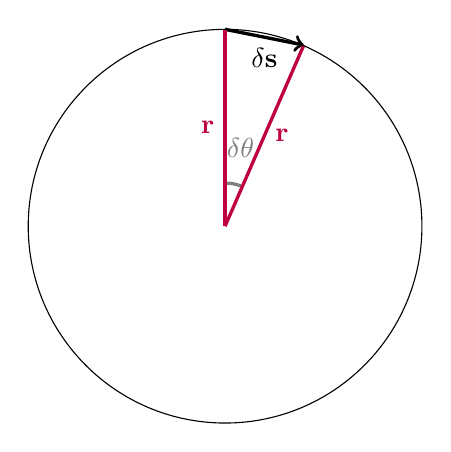
\begin{tikzpicture}[remember picture]
		\draw [very thick,gray](0.225,0.5) arc (65:92:0.5);
		\draw[very thick, black, ->] (0,2.5) -- node[below] {$\mathbf{\delta s}$}  (1,2.3);
		\draw[very thick, purple, -] (0,0) -- node[left] {$\mathbf{r}$} (0,2.5);
		\draw[very thick, purple, -] (0,0) -- node[right]{$\mathbf{r}$} (1,2.3);
		\draw [gray](-0.1,1) node[right]{$\delta\theta$};

		\draw (0,0) circle (2.5cm);
		\end{tikzpicture}
	\end{center}
	\caption{}
\end{figure}

From the definition of the radian, in a small time interval $\delta t$ we can say that the displacement of the rotating object is $\delta s \approx r\delta\theta$ (see figure 10.1), and hence in the limit as we make the time interval smaller that means $v=\frac{ds}{dt} = r\frac{d\theta}{dt}=r\omega$

\begin{example}
	Calculate the linear velocity of the Earth relative to the sun, given the Earth-Sun distance is 1.5 x $10^{11} $m

\answer First calculate the angular velocity of the Earth. It performs a complete orbit (ie $2\pi$ radians) in 1 year, so $\omega= \frac{2\pi}{365\times24\times3600}$

Then $v=r\omega$ = 30000 $ms^{-1}$
\end{example}
\spec{
	Derive, recall and use the equations for centripetal acceleration $a = \frac{v ^{2}}{r}$ and $a = r\omega ^{2}$
}

Since acceleration is defined as change in velocity, we can see from the following diagram (figure 10.2) that the velocity change when a uniformly rotating object moves through a small angle $\delta\theta$ can be written as $\delta v = v\delta\theta$ since the magnitudes of the initial and final velocity are both equal to v.
\\
\\

\begin{figure}[h]
	\begin{center}
		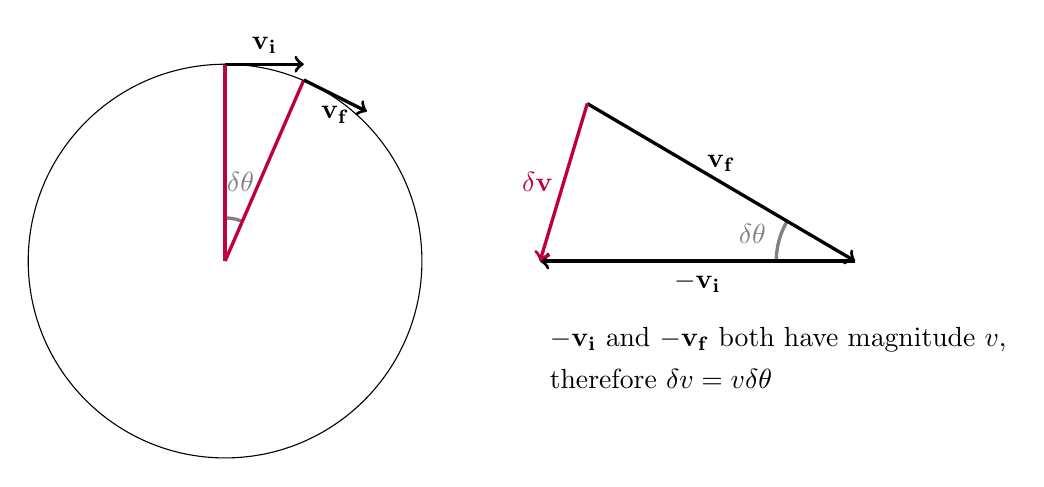
\begin{tikzpicture}
		\draw [very thick,gray](0.225,0.5) arc (65:92:0.5);
		\draw[very thick, black, ->] (0,2.5) -- node[above] {$\mathbf{v_i}$}  (1,2.5);
		\draw[very thick, black, ->] (1,2.3) -- node[below] {$\mathbf{v_f}$}  (1.8,1.9);
		\draw[very thick, purple, -] (0,0) -- node[left] {} (0,2.5);
		\draw[very thick, purple, -] (0,0) -- node[right] {} (1,2.3);
		\draw [gray](-0.1,1) node[right]{$\delta\theta$};

		\draw (0,0) circle (2.5cm);

		\draw [very thick,gray](7,0) arc (180:150:1);

		\draw[very thick, black, ->] (8,0) -- node[below] {$\mathbf{-v_i}$}  (4,0);
		\draw[very thick, black, ->] (4.6,2) -- node[above] {$\mathbf{v_f}$}  (8,0);
		\draw[very thick, purple, ->] (4.6,2) -- node[left] {$\mathbf{\delta v}$} (4,0);
		\draw [gray](6.4,0.35) node[right]{$\delta\theta$};

		\draw [black](4,-1) node[right]{$\mathbf{-v_i}$ and $\mathbf{-v_f}$ both have magnitude $v$, };
		\draw [black](4,-1.5) node[right] {therefore $\delta v = v \delta\theta$};
		\end{tikzpicture}
	\end{center}
	\caption{}
\end{figure}


The acceleration is therefore $a\approx\frac{v\delta\theta}{\delta t}$ and as we let $\delta t\rightarrow0$ we get $a=v\frac{d\theta}{dt}=v\omega$.
\\
since $v=r\omega$ we also get $a=\frac{v^2}{r}=r\omega^2$



\spec{Recall that F = ma applied to circular motion gives resultant $F=\frac{mv^2}{r}$}

Since $a = \frac{v ^{2}}{r}$ and $F=ma$ we can combine these to give $F=\frac{mv^2}{r}$. This can be very useful for example when combined with Newton's law of Gravity to explain planetary orbits etc.
\\
\\

\begin{example}
	Show that, for a circular orbit, the time period squared is proportional to the radius cubed.

 	\answer Start by equating $F=mr\omega^2$ with $F= \frac{GMm}{r^2}$ (we can ignore the minus sign)
\\

$mr\omega^{2}= \frac{GMm}{r^2}$
\\
\\
Then rearrange and cancel $m$ to find
\\
\\
$r^{3}=\frac{GM}{\omega^2}$
\\
\\
then using $\omega=\frac{2\pi}{T}$ we get
\\
\\
$r^{3}=\frac{GM}{4\pi^{2}}T^2$

\end{example}

\spec{Describe qualitatively the motion of a rigid solid object under the influence of a single force in terms of
linear acceleration and rotational acceleration.}

When a rigid solid object has a single force applied to it, it may just result in linear acceleration, if the force acts through the centre of mass of the object. However it is more likely that the force will not act through this point, and therefore also cause some rotational acceleration, causing the object's angular velocity to change.
\\
\\
The remaining sections in this chapter deal with how we describe this rotational acceleration, but it should be noted that they are asterisked sections so will only form part of section 2 of paper 3.

\
\spec{*Recall and use $I = \Sigma mr^2$ to calculate the moment of inertia of a body consisting of three or fewer point
particles fixed together}

The moment of inertia of a body is the rotational analogue of mass, and basically describes how resistant an object is to angular acceleration when a torque is applied (in the same way that mass describes how resistant an object is to accelerating linearly when a force is applied...)

A point mass $m$ at a distance $r$ from an axis of rotation will have Moment of Inertia $I=mr^2$

More generally the moment of inertia is the sum of all the $mr^2$ values for all the point masses that make up an object. For a small number of particles this can just be found by adding the values of individual moments of inertia.
\\
\spec{*Use integration to calculate the moment of inertia of a ring, a disk and a rod}

For more complex bodies, the summing of moments of inertia needs to be done by setting up an integration. This is acheived by summing moments of inertia for a series of small sections of the object, strips or rings of thickness $\delta x$ say, and using the fact that as $\delta x \rightarrow0$ the sum $\Sigma \delta x \equiv \int dx$

As an example, consider a disk of radius r , thickness t and density $\rho$. The moment of inertia about its central axis could be found by splitting it up into rings of radius $x$ and thickness $\delta x$. See figure 10.3.
\\
\begin{figure}[h]
	\begin{center}
		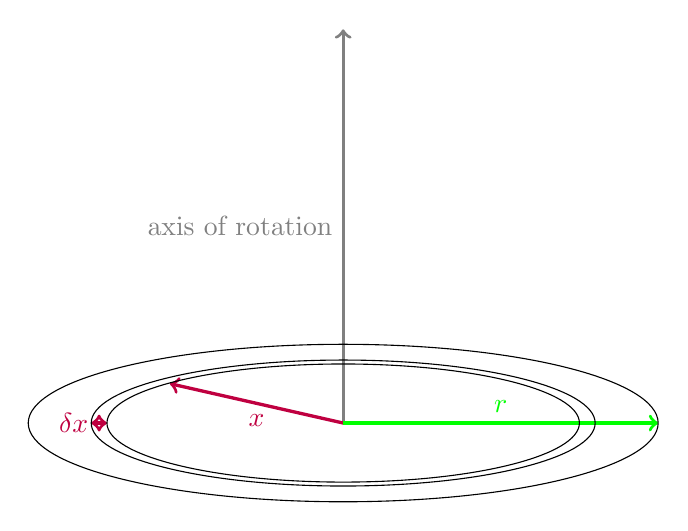
\begin{tikzpicture}
		\draw[very thick, gray, ->] (0,0) -- node[left] {{axis of rotation}}  (0,5);

	\draw[very thick, purple, ->] (0,0) -- node[below] {$x$} (-2.2,0.5);
	\draw[very thick, purple, <->] (-3.2,0) -- node[left] {$\delta x$} (-3.0,0);
	\draw[very thick, green, ->] (0,0) -- node[above] {$r$} (4.0,0);
		\draw (0,0) ellipse (4cm and 1cm);
		\draw (0,0) ellipse (3cm and 0.75cm);
		\draw (0,0) ellipse (3.2cm and 0.8cm);
		\end{tikzpicture}
		\caption{}
	\end{center}
\end{figure}

Each ring has moment of inertia equal to its mass multiplied by $x^2$, as all the particles in it have (approximately) the same distance from the axis.\footnote{This can be proved by another, much simpler, sum. If you imagine the ring as the sum of many small points of mass $\delta m$ each at the same radius $r$, the moment of inertia becomes $\Sigma r^{2}\delta m$ which is the same as $r^{2}\Sigma \delta m$ and hence $I=mr^2$}
\\

Hence $I_{ring}= (2\pi x t \rho\delta x )x^2 = 2\pi \rho x^{3} \delta x$
\\

To find the moment of inertia of the disk, we sum all the rings and let their size $\delta x$ tend to 0.


$I_{disk}= \Sigma 2\pi \rho x^{3} \delta x$
\\

$I_{disk}= \int\displaylimits_0^r 2\pi \rho  t x^{3}\delta x $
\\

giving
\\

$I_{disk} = \frac{2\pi\rho t r^4}{4}$
\\

which is equal to

$I_{disk} = \frac{mr^2}{2}$
\\

Other objects would be derived in a similar way. You should get $I=\frac{mr^2}{3}$ for a rod rotating about one end, and $I =\frac{mr^2}{12}$ for a rod rotating about its centre of mass.
\\

\spec{*Deduce equations for rotational motion by analogy with Newton’s laws for linear motion, including
$E =\frac{1}{2}I\omega ^2$, $ L = I\omega$ and $\Gamma=I \frac{d\omega}{dt}$}

Here is a table outlining the analogies between linear and rotational moton:
\\

\begin{center}
	\begin{tabular}{||c c||}
		\hline
		\textbf{Linear Motion} & \textbf{Rotational Motion}\\ [0.5ex]
		\hline\hline
		 Mass m &Moment of Inertia I\\
		\hline
		linear velocity v &Angular velocity $\omega$\\
		\hline
		Force F & Torque $\Gamma$ \\
		\hline
		Linear Momentum p  & Angular Momentum L \\
		\hline
		$p=mv$ & $ L = I\omega$  \\
		\hline
		$F=ma =m\frac{dv}{dt}$ & $\Gamma=I \frac{d\omega}{dt}$ \\
		\hline
		$KE_{linear}=\frac{1}{2}mv^2$ & $KE_{rotational} =\frac{1}{2}I\omega ^2$\\ [1ex]
		\hline
	\end{tabular}
\end{center}



\
\spec{*Apply the laws of rotational motion to perform kinematic calculations regarding a rotating object when
the moment of inertia is given.}

\begin{example}
	The moment of inertia of a large flywheel in a factory is 60 kgm$^2$. Calculate how long it would take the flywheel to obtain an angular velocity of 6.0 rad s$^{-1}$ when a torque of 24 Nm was applied.
	\answer
First use $\Gamma=I \frac{d\omega}{dt}$ to find the angular acceleration:

$\frac{d\omega}{dt}=\frac{\Gamma}{I}=\frac{24}{60}= 0.4$ rad s$^{-2}$

Then the time taken will be

$T=\frac{6}{0.4}=15$ seconds
\end{example}
\end{document}
